\documentclass[pdflatex,11pt]{aghdpl}

\usepackage[polish]{babel}
\usepackage[utf8]{inputenc}
\usepackage[T1]{fontenc}

% dodatkowe pakiety
\usepackage{enumerate}
\usepackage{pdfpages}
\usepackage{afterpage}
\usepackage{pdflscape}
%\usepackage{rotating}

\graphicspath{{./img/}}
%\usepackage{subfigure} %kilka obrazkow w ramach jednego figure

%---------------------------------------------------------------------------

\author{Marta~Drabarczyk, Krzysztof~Kutt, Michał~Nowak, Aleksandra~Sikora, Olga~Zachariasz}
\titlePL{Wirtualne Warsztaty}
\thesistypePL{Zarządzanie Projektami Informatycznymi}
\date{2012}
\departmentPL{Katedra Automatyki}
\facultyPL{Wydział Elektrotechniki, Automatyki, Informatyki i Elektroniki}
\setlength{\cftsecnumwidth}{10mm}

%---------------------------------------------------------------------------

\begin{document}

\titlepages

\tableofcontents
\clearpage

\chapter{Wykład 2. Metodologia zarządzania projektami w przedsiębiorstwie informatycznym}

\section{Model wybranego procesu}
% strona 43

Ten wirtualny warsztat jest beznadziejny.

% ===========================================================================

\section{Produkty, procesy, projekty}
% strona 78

Ten wirtualny warsztat jest beznadziejny.

% ===========================================================================

\section{Role w przedsiębiorstwie}
% strona 90

Ten wirtualny warsztat jest beznadziejny.



\chapter{Wykład 3. Środowisko zarządzania projektami w przedsiębiorstwie}

\section{Strategia firmy}
% strona 8

\subsection*{Wizja}

Wizją naszego przedsiębiorstwa jest stworzenie systemów wspierających zarządzanie projektami informatycznymi.

\subsection*{Misja}

Nasza firma dąży do tego, aby być najlepszym pod względem jakości i niezawodności dostawcą oprogramowania do zarządzania projektami informatycznymi na rynku.

\subsection*{Cele strategiczne}

Plan dwuletni naszego przedsiębiorstwa zakłada:
\begin{itemize}
\item stworzenie sztandarowego produktu firmy, który zapewni rozpoznawalność marki oraz stały dochód na poziomie 200 000 zł miesięcznie,
\item wypuszczenie na rynek dwóch kolejnych produktów,
\item osiągnięcie sprzedaży na poziomie 50 licencji na kwartał,
\item ekspansja działalności firmy na rynki czeski i słowacki.
\end{itemize}

\subsection*{Zasady (Wartości)}

\begin{itemize}
\item Dobre traktowanie pracowników
\item Najwyższa jakość produktów
\item Bezstronność
\item Niezależność od innych przedsiębiorstw
\end{itemize}

% ===========================================================================

\section{Strategia rozwoju firmy}
% strona 14

Nasza firma w swojej działalności stawia na innowacyjność. Działalność operacyjna obejmuje tworzenie oprogramowania wspierającego zarządzanie projektami w przedsiębiorstwach. Jako firma wyznaczamy nowe kierunki działania i eksperymentujemy z nowymi technologiami. Staramy się zrozumieć potrzeby naszego Klienta. Współpraca biznesowa z Klientem jest bardzo ważnym czynnikiem rozwoju firmy. 
Jako pracodawca staramy się inwestować w młody i ambitny zespół. Potrzeby naszego pracownika są dla nas bardzo ważne, dlatego szczególną uwagę zwracamy na środowisko pracy, stałe zatrudnienie oraz opiekę socjalną pracownika. Wierzymy, że zadowolony pracownik to wydajny pracownik, dzięki, któremu możliwy jest sukces firmy.  

\textbf{Powiązania strategii ze szkołami zarządzania strategicznego:}

\textit{Szkoła zasobów i kompetencji} – nacisk na dbanie o pracownika i przeświadczenie, że praca jednostki składa się na sukces całego przedsięwzięcia.

\textit{Szkoła planistyczna} – strategia stworzona na bazie analizy SWOT.


% ===========================================================================

\section{Sieć zależności korzyści}
% strona 37

Ten wirtualny warsztat jest beznadziejny.

% ===========================================================================

\section{Zarządzanie portfelem projektów}
% strona 47

Ten wirtualny warsztat jest beznadziejny.

% ===========================================================================

\section{Czynniki środowiskowe}
% strona 78

\subsection*{Wewnętrzne}

\begin{itemize}
\item Dobre traktowanie pracowników
\end{itemize}

\subsection*{Związane z partnerami}

\begin{itemize}
\item Dobre traktowanie pracowników
\end{itemize}

\subsection*{Zewnętrzne}

\begin{itemize}
\item Dobre traktowanie pracowników
\end{itemize}


\chapter{Wykład 4. Zarządzanie wiedzą w przedsiębiorstwie}

\section{Wiedza potrzebna w projekcie}
% strona 19

\subsection*{Wiedza deklaratywna:}
\begin{itemize}
\item Składniki metodyki PMBOK:
\begin{itemize}
\item pojęcia
\item role
\item procesy
\item dokumenty
\item obszary wiedzy
\end{itemize}
\item Istniejące rozwiązania problemu
\item Technologie, z których można skorzystać
\end{itemize}

\subsection*{Wiedza strukturalna:}
\begin{itemize}
\item struktura zależności pomiędzy elementami metodyki PMBOK
\item struktura bazy danych spełniającej wymagania
\item struktura oprogramowania, które chcemy wytworzyć
\end{itemize}

\subsection*{Wiedza proceduralna:}
\begin{itemize}
\item jak wygląda przepływ danych w projekcie
\item jakie są przypadki użycia
\item kiedy są tworzone poszczególne dokumenty
\item jak można wykorzystać dostępne technologie
\end{itemize}

% ===========================================================================

\section{Procesy wykorzystania produktu projektu}
% strona 34

\begin{figure}[!h]
\centering
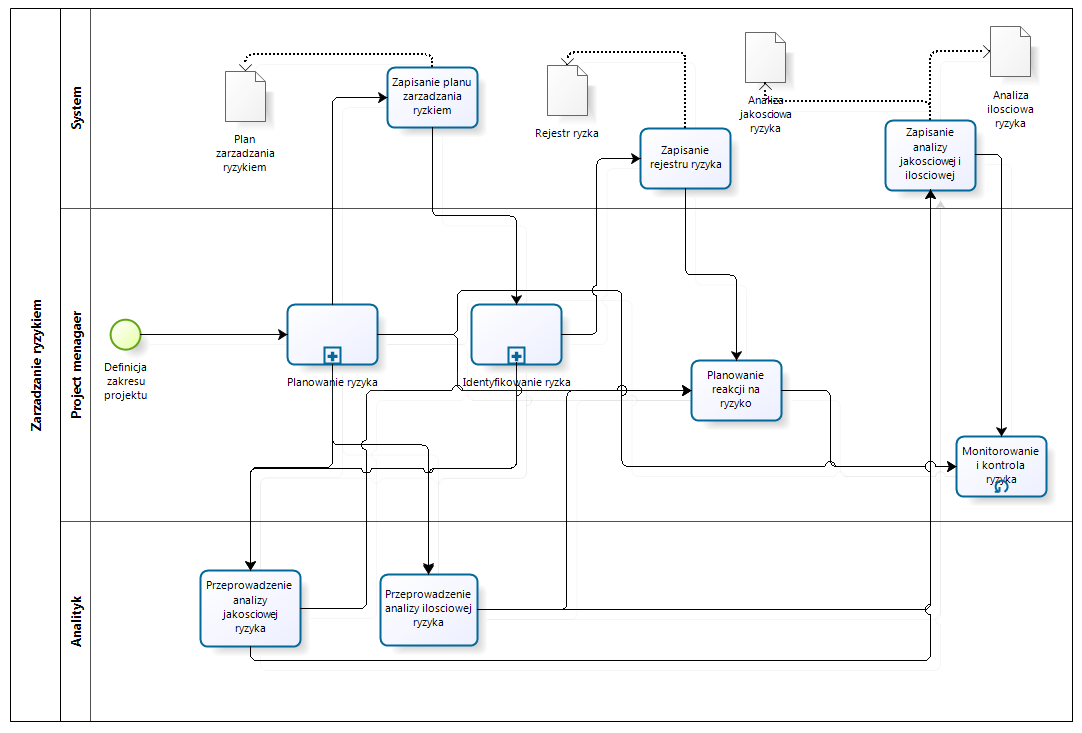
\includegraphics[width=1.1\textwidth]{zarzadzanieRyzykiem.png}
\caption{Zarządzanie ryzykiem}
\label{fig:zarzadzanieRyzykiem}
\end{figure}

\begin{figure}[!h]
\centering
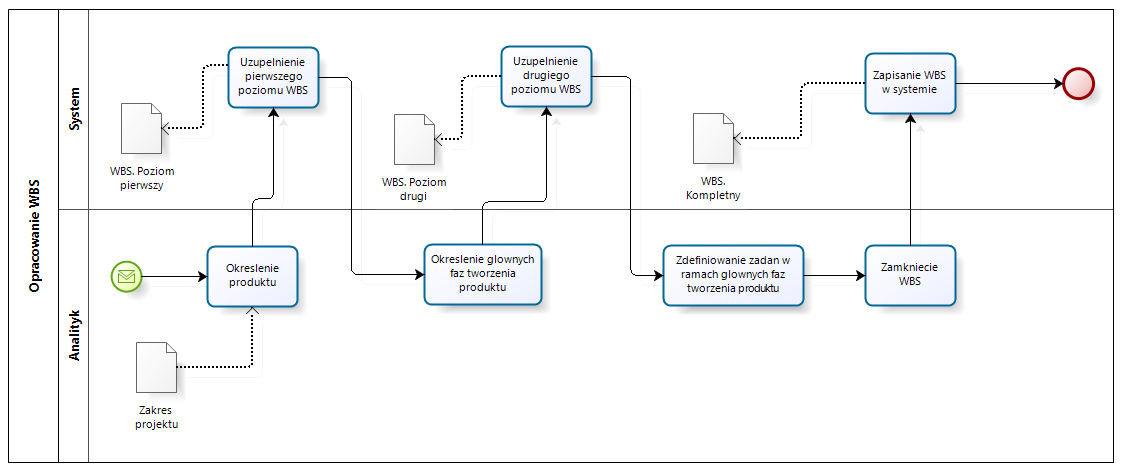
\includegraphics[width=1.1\textwidth]{opracowywanieWBS.png}
\caption{Tworzenie WBS}
\label{fig:opracowanieWBS}
\end{figure}

\clearpage

% ===========================================================================

\section{Systemy informatyczne do zarządzania wiedzą}
% strona 59

Do zarządzania wiedzą w przedsiębiorstwie można wykorzystywać różnorakie systemy. Ich najważniejszymi zadaniami są:
\begin{itemize}
\item Gromadzenie wiedzy
\item Systematyzacja wiedzy
\item Dystrybucja wiedzy
\end{itemize}

Przedstawione zostaną tutaj najważniejsze i najciekawsze z dostępnych programów.

\begin{itemize}
\item \textbf{Portale korporacyjne}. Najczęściej służą do jednokierunkowego przepływu informacji: od firmy do pracowników / klientów. Można rozszerzyć je o fora, albo dodać każdemu użytkownikowi możliwość dodawania informacji na portalu, jednak nie jest to skuteczny sposób na dwukierunkową komunikację.\\
\textbf{Przykładowe programy:} \textit{Drupal} (producent: Dries Buytaert), \textit{Joomla!} (producent: The OSM Development Team).

\item \textbf{Listy mailingowe}. Pozwalają na definiowanie grup, w ramach których wymieniane są informacje. Pozwala to na stworzenie prostego systemu przesyłania informacji w poszczególnych projektach (dla każdego projektu osobna lista). Można skorzystać z zewnętrznych serwerów, bądź zainstalować aplikację na firmowym sprzęcie. Są łatwo dostępne dla pracowników, dzięki możliwości obsługi przez przeglądarkę internetową. \\
\textbf{Przykładowe programy:} \textit{Google Groups} (zewnętrzny serwer), \textit{Majordomo} (producent: Great Circle Associates, do instalacji na własnym serwerze).

\item \textbf{Systemy zarządzania dokumentami (DMS)}. Umożliwiają gromadzenie i przeszukiwanie bazy dokumentów. Pozwalają na regulację dostępu poszczególnych osób do poszczególnych plików. Udostępniają również wersjonowanie wszystkich plików.\\
\textbf{Przykładowe programy:} \textit{Microsoft SharePoint}, \textit{OpenKM} (producent: GIT Consultors S.L.).

\item \textbf{Systemy automatyzacji pracy (workflow)}. Oprogramowanie takie pozwala na określenie ról poszczególnych osób w przetwarzaniu dokumentów oraz stanów pośrednich dokumentów. Procesy workflow przedstawia się zwykle w postaci grafu. \\
\textbf{Przykładowe programy:} \textit{Route} (OpenSource, tworzony przez Route Team), \textit{ONE Workflow} (producent: BeOne Sp. z o.o.).

\item \textbf{Bazy danych i hurtownie danych}. Pozwalają gromadzić bieżące dane, a także dane historyczne, na podstawie których przygotowywane są raporty i zestawienia.\\
\textbf{Przykładowe programy:} \textit{Microsoft Access}, \textit{LibreOffice Base} (producent: The Document Foundation).

\item \textbf{Systemy analizy danych (data mining)}. Pozwalają na odkrywanie powiązań pomiędzy danymi zapisanymi w bazach danych i hurtowniach danych.\\
\textbf{Przykładowe programy:} \textit{Oracle Data Mining}, \textit{Statistica: Data Miner} (producent: StatSoft).

\item \textbf{Wideokonferencje}.\\
\textbf{Przykładowe programy:} \textit{Skype} (producent: Microsoft), \textit{AQQ} (producent: CT Creative Team S.A.).

\item \textbf{Help-desk}. System umożliwiający zapisywanie i udostępnianie wiedzy zgromadzonej w procesie rozwiązywania problemów. W najprostszej wersji może to być podstrona portalu przedsiębiorstwa z listą najczęściej zadawanych pytań (FAQ).\\
\textbf{Przykładowe programy:} \textit{HelpTrac} (producent: Monarch Bay Software, Inc), \textit{Control-F1} (producent: CA Technologies).

\item \textbf{E-learning}. Nauka na odległość. Systemy pozwalające na przyswajanie wiedzy i kontakt z ekspertami poprzez internet.\\
\textbf{Przykładowe programy:} \textit{Moodle} (producent: Moodle Community), \textit{Chamilo} (producent: Chamilo Community).

\item \textbf{Systemy Wiki}. Typ witryn internetowych, w których treść można tworzyć i zmieniać w prosty i szybki sposób, z poziomu przeglądarki internetowej. Nie wymagana jest znajomość nawet HTMLa, ponieważ wykorzystywany jest specjalny język znaczników.\\
\textbf{Przykładowe programy:} \textit{MediaWiki} (producent: Wikimedia Foundation), \textit{DokuWiki} (producent: Andreas Gohr).

\item \textbf{Systemy ekspertowe}. Zawierają bazę wiedzy oraz reguły wnioskowania w celu rozwiązywania problemów.\\
\textbf{Przykładowe programy:} \textit{HeKaTe} (projekt rozwijany w Katedrze Automatyki), \textit{CLIPS} (stworzony przez NASA, aktualnie rozwijany przez CLIPS Expert System Group).

\end{itemize}

\clearpage

% ===========================================================================

\section{Mapa umysłu dla systemu zarządzania wiedzą}
% strona 70

\begin{figure}[!h]
\centering
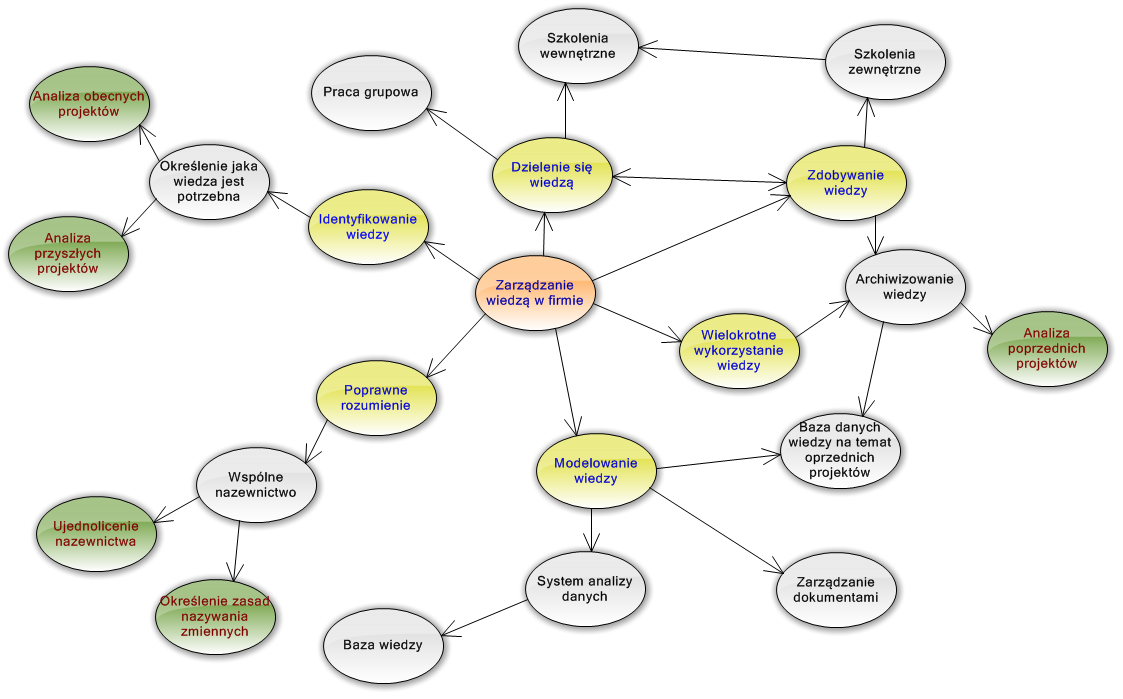
\includegraphics[width=\textwidth]{mapaMysli.png}
\caption{Mapa myśli}
\label{fig:mapaMysli}
\end{figure}

%\clearpage

% ===========================================================================

\section{Przegląd praktyk OPM3}
% strona 89

Praktyki OPM3, które powinny być w firmie:

\begin{enumerate}
\item Integrate PMBOK Guide Knowledge Areas; z racji związania projektu z metodyką PMBOK
\item Project Team Development Process Measurement; w związku z pracą zespołową nad projektem
\item Project Risk Response Planning Process Control; związane z występowaniem ryzyka
\end{enumerate}

Praktyki OPM3 zbędne w firmie:

\begin{enumerate}
\item Know Inter-Project Plan; w trakcie trwania projektu nie będą prowadzone równolegle inne projekty
\item Optimize Portfolio Management; brak portfolio
\item Track the Return of Investment; projekt nie jest inwestycją firmy
\end{enumerate}


\chapter{Wykład 5. Zarządzanie projektami wg metodyki PMBOK}

\section{Analiza wartości}
% strona 14
\subsection*{Dokonaj analizy wartości PMBOK, które mogą być przydatne w projekcie.}

Wartości, które mogą być przydatne w projekcie:
\begin{itemize}
\item profesjonalizm działania i etyka zawodowa, 
\item kompetentna kadra zarządzająca projektem ,
\item profesjonalne zachowanie w trakcie realizacji projektu,
\item ogólny i globalny charakter metodyki,
\item skalowanie metodyki, 
\item dostarczenie klientowi projektu dokładnie takiego jakiego wymagał,
\item wartościowanie wymagań,
\item plan i pro aktywne działanie,
\item planowanie kroczące i poprawa planów,
\item zintegrowane zarządzanie zmianą. 
\end{itemize}

\subsection*{Wyznacz zasady i wartości dla Twojego projektu.}

Zasady i wartości dla naszego projektu:
\begin{itemize}
\item ustalone reguły zachowania i postępowania,
\item konsekwentne postępowanie według przyjętego plany,
\item omawianie potencjalnych konfliktów,
\item wspólne rozwiązywanie problemów,
\item trzymanie się ustalonego sposobu raportowania, jak najszybsze informowanie o zmianach,
\item spotkania, które pozwolą na przedstawienie różnych punktów widzenia.
\end{itemize}

% ===========================================================================

\section{Role i struktury organizacyjne}
% strona 51

Role w PMBOK:
\begin{enumerate}
\item	Wykonawca projektu (Project Performer) – osoba/organizacja odpowiedzialna za projekt.
	\begin{enumerate}
	\item	Zespół projektowy (Project Team) – zespół składający się zarówno z osób zajmujących się zarządzaniem projektem jak i  osób wykonujących pracę nad produktem wyjściowym.  Zespół projektowy wykonując swoje obowiązki dąży do dostarczenia produktu.
		\begin{enumerate}
		\item	Zespół rozwijający project (Project Development Team) – zespół odpowiedzialny za wykonywanie pracy związanej z wytworzeniem produktu i spełnieniem narzuconych wymagań.
		\item	Zespół zarządzania projektem (Project Management Team) – zespół odpowiedzialny za planowanie, kontrolowanie i monitorowanie pracy nad projektem. Zespół wspiera Kierownika projektu dostarczając mu niezbędnych informacji uzyskanych podczas procesu monitorowania projektu.
		\end{enumerate}
	\item	Kierownik projektu (Project Manager) – jest odpowiedzialny za planowanie i organizację pracy podczas realizacji projektu. Zarządza wszystkimi działaniami codziennymi. PM odpowiada za dostarczenie klientowi produktu. Jest to osoba reprezentująca projekt na zewnątrz oraz odpowiadająca za jego sukces.
	\item	Kierownik funkcjonalny (Functional Manager) – jest odpowiedzialny za zarządzanie szeroko pojętym biznesem, czyli finansami, kontraktami oraz zasobami ludzkimi.
	\item	Rada kontroli zmian (Change Control Board) – grupa zajmująca się kontrolowaniem zmian w projekcie. Grupa ma prawo zarówno do akceptacji jak i odrzucenia zmian w projekcie. 
	\item	Biuro zarządzania projektem (PMO – Project Management Office) – jednostka wspierająca zarządzaniem projektem w przedsiębiorstwie. Biuro projektowe wspiera projekt pod kątem administracyjnym – zarządza dokumentacją, zasobami ludzkimi i przebiegiem projektu.
	\end{enumerate}
\item	Klient (Customer) – kupujący produkt lub usługę wytworzone podczas projektu.  
\item	Użytkownik (User) – rodzaj klienta nie będącego bezpośrednim nabywcą produktu. Użytkownik korzysta  z produktu.
\item	Inwestor (Sponsor) – osoba (lub grupa osób) dostarczająca środków finansowych na realizację projektu, mająca znaczny wpływ na zakres projektu. Inwestor jest osobą odpowiedzialną za akceptację produktu.

Zleceniodawca (Project Customer) – typ inwestora zlecającego wykonanie projektu w formie kontraktu. 
\item	Sprzedawca (Seller) – osoba/organizacja/przedsiębiorstwo sprzedająca/e produkt lub usługę. Sprzedawca nie musi być wytwórcą produktu.
\end{enumerate}

W PMBOK nie ma jasno określonej definicji struktury organizacyjnej. Struktury organizacyjne tworzy się w celu realizacji wyspecyfikowanych zadań. Można wyróżnić kilka typów struktur organizacyjnych:
\begin{itemize}
\item	Projektowa – podział per projekt. Kierownik projektu ma silną władzę. 
\item	Funkcjonalna – podział per funkcja. Działy funkcjonalne kierowane przez specjalistów, pracownik podlega więcej niż jednemu kierownikowi.
\item	Macierzowa (Matrix) – połączenie struktury projektowej i funkcjonalnej.
\end{itemize}


\textbf{Wyznacz role i struktury organizacyjne dla Twojego projektu:}


W naszym projekcie występują następujące role:
\begin{itemize}
\item Kierownik Projektu
\item Zespół projektowy
\item Rada kontroli zmian
\item Inwestor
\item Użytkownik
\end{itemize}

\clearpage

Przyjmujemy projektową strukturę organizacyjną:
\begin{figure}[!ht]
\begin{center}
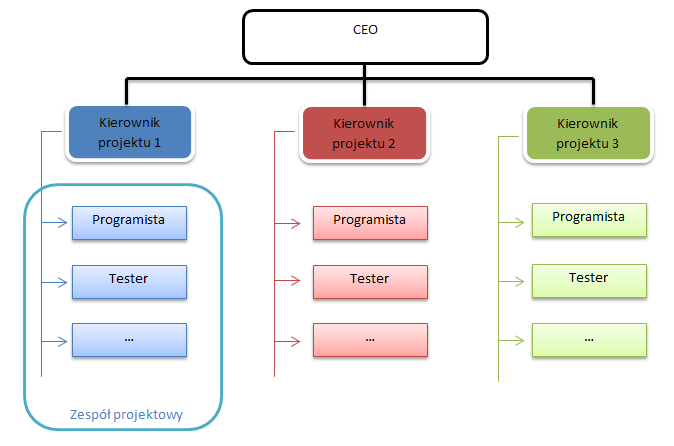
\includegraphics[width=\textwidth]{struktura_org.png}
\caption[Struktura organizacyjna]{Struktura organizacyjna}
\label{rysunekProces}
\end{center}
\end{figure}





\chapter{Wykład 6. Systematyczny opis metodyki SCRUM w zarządzaniu projektami}

\section{Czy warto wprowadzić metodykę SCRUM?}
% strona 89

Ten wirtualny warsztat jest beznadziejny.



\chapter{Wykład 7. Zintegrowane zarządzanie projektem informatycznym}

\section{Sukces projektu}
% strona 23

Ten wirtualny warsztat jest beznadziejny.

% ===========================================================================

\section{Rozpoczęcie projektu}
% strona 28

Ten wirtualny warsztat jest beznadziejny.

% ===========================================================================

\section{Karta projektu}
% strona 33

Ten wirtualny warsztat jest beznadziejny.

% ===========================================================================

\section{Plan zarządzania projektem wg B.A.R.F.}
% strona 44

Ten wirtualny warsztat jest beznadziejny.



\chapter{Wykład 8. Zarządzanie zakresem projektu i produktu w projekcie informatycznym}

\section{Wymagania}
% strona 16

\begin{table}[htb]
\centering
\begin{tabular}{r|c c c|p{10.5cm}} 
Lp. & TC1 & TC2 & TC3 & Wymaganie \\
\hline
1 & + &  &  & Użytkownik może utworzyć konto \\
2 & + & + & + & Użytkownik może się zalogować \\
3 &  & + &  & PM może tworzyć projekty \\
4 &  & + &  & PM może otwierać procesy \\
5 &  &  &  & PM może zamykać procesy \\
6 &  &  & + & Użytkownik może zamykać zadania \\
7 &  & + &  & PM może dodawać/usuwać/modyfikować nowe zadania \\
8 &  & + &  & PM może przypisywać zadania do użytkowników \\
9 & + &  &  & Administrator oraz PM mogą nadawać role \\
10 & + &  &  & Administrator może weryfikować nowych użytkowników \\
11 & + &  &  & Administrator może przeglądać listę oczekujących \\
12 &  & + & + & Użytkownik oraz PM może dodać/edytować dokument \\
13 &  &  & + & PM może usuwać dokument \\
14 & + & + &  & System umożliwia ograniczenie dostępu do zasobów \\
15 &  & + &  & System tworzy domyślne zadania dla każdego procesu \\
\end{tabular}
\caption{\textbf{Macierz zależności wymagań}}
\label{tab:macierzWymagan}
\end{table}


\textbf{TC 1}
\begin{enumerate}
\item Nowy pracownik zakłada konto
\item Administrator przegląda listę użytkowników i znajduje to konto
\item Administrator weryfikuje je
\item Administrator nadaje mu odpowiednią rolę (np programista)
\item Nowy pracownik może się zalogować
\item Nowy pracownik nie ma dostępu do kluczowych dokumentów (dopóki nie zostanie mu przydzielony odpowiedni dostęp)
\end{enumerate}


\textbf{TC 2}
\begin{enumerate}
\item PM loguje się do systemu
\item PM tworzy nowy projekt
\item System automatycznie generuje podstawowe procesy i szablony dokumentów
\item PM otwiera proces otwarcia
\item PM edytuje dokument otwarcia (uzupełnia wygenerowany szablon)
\item PM modyfikuje informacje dotyczące analizy wymagań (określa deadline)
\item PM przyporządkowuje dwóch analityków do edycji analizy wymagań
\item PM ukrywa dostęp do dokumentu analizy wymagań przed innymi użytkownikami
\end{enumerate}


\textbf{TC 3}
\begin{enumerate}
\item Użytkownik loguje się do systemu
\item Użytkownik oznacza swoje ostatnie zadanie jako wykonane
\item Użytkownik przypadkiem wrzuca list miłosny do repozytorium
\item PM kasuje zbędny dokument
\item PM zamyka proces realizacji
\end{enumerate}



% ===========================================================================

\section{Mapa umysłu dla zakresu projektu}
% strona 22

Ten wirtualny warsztat jest beznadziejny.

% ===========================================================================

\section{Diagram SPP}
% strona 59

Ten wirtualny warsztat jest beznadziejny.



\chapter{Wykład 9. Zarządzanie czasem w projekcie informatycznym}

\section{SPP uwzglęniający plan kont kosztowych projektu}
% strona 34

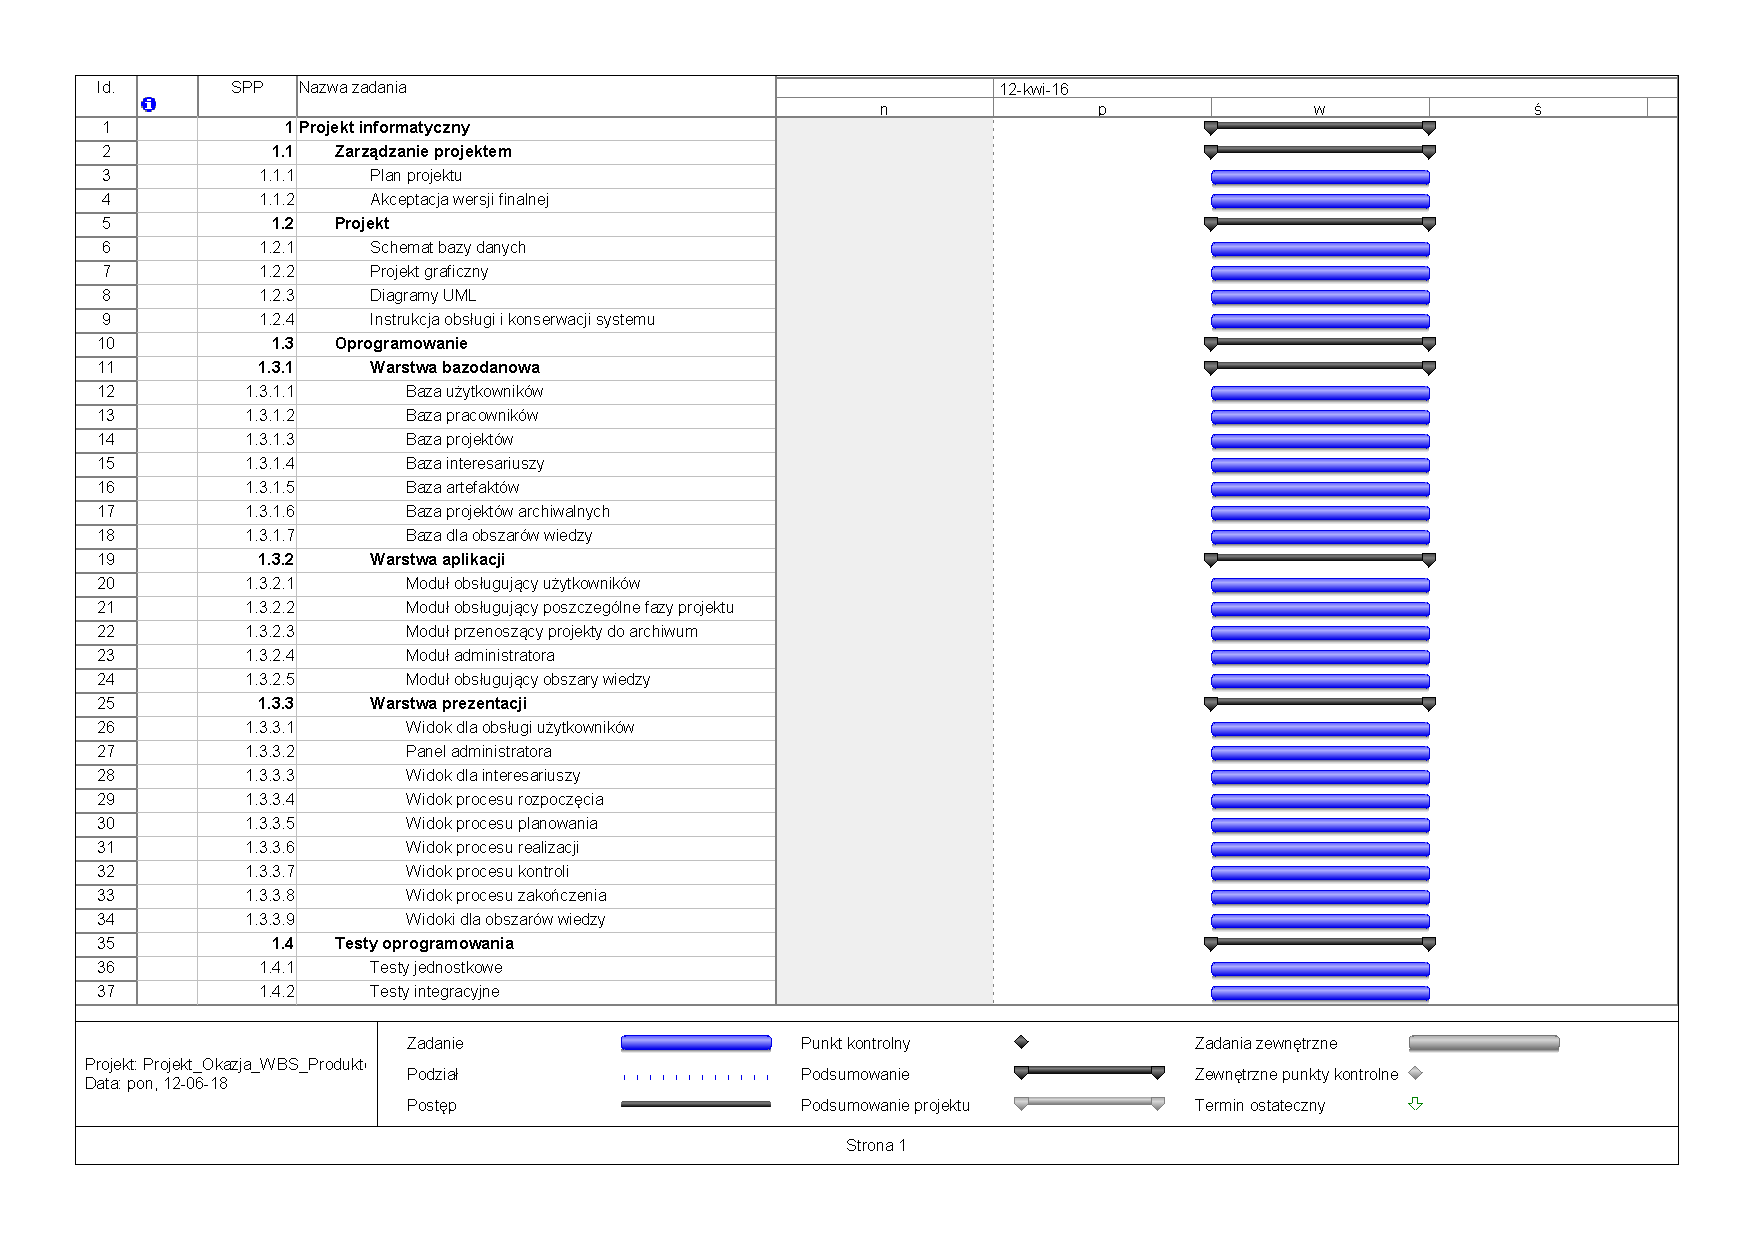
\includepdf[nup=1x2,pages=-]{diagramSPP.pdf}

% ===========================================================================

\section{Harmonogram w MS Project}
% strona 35

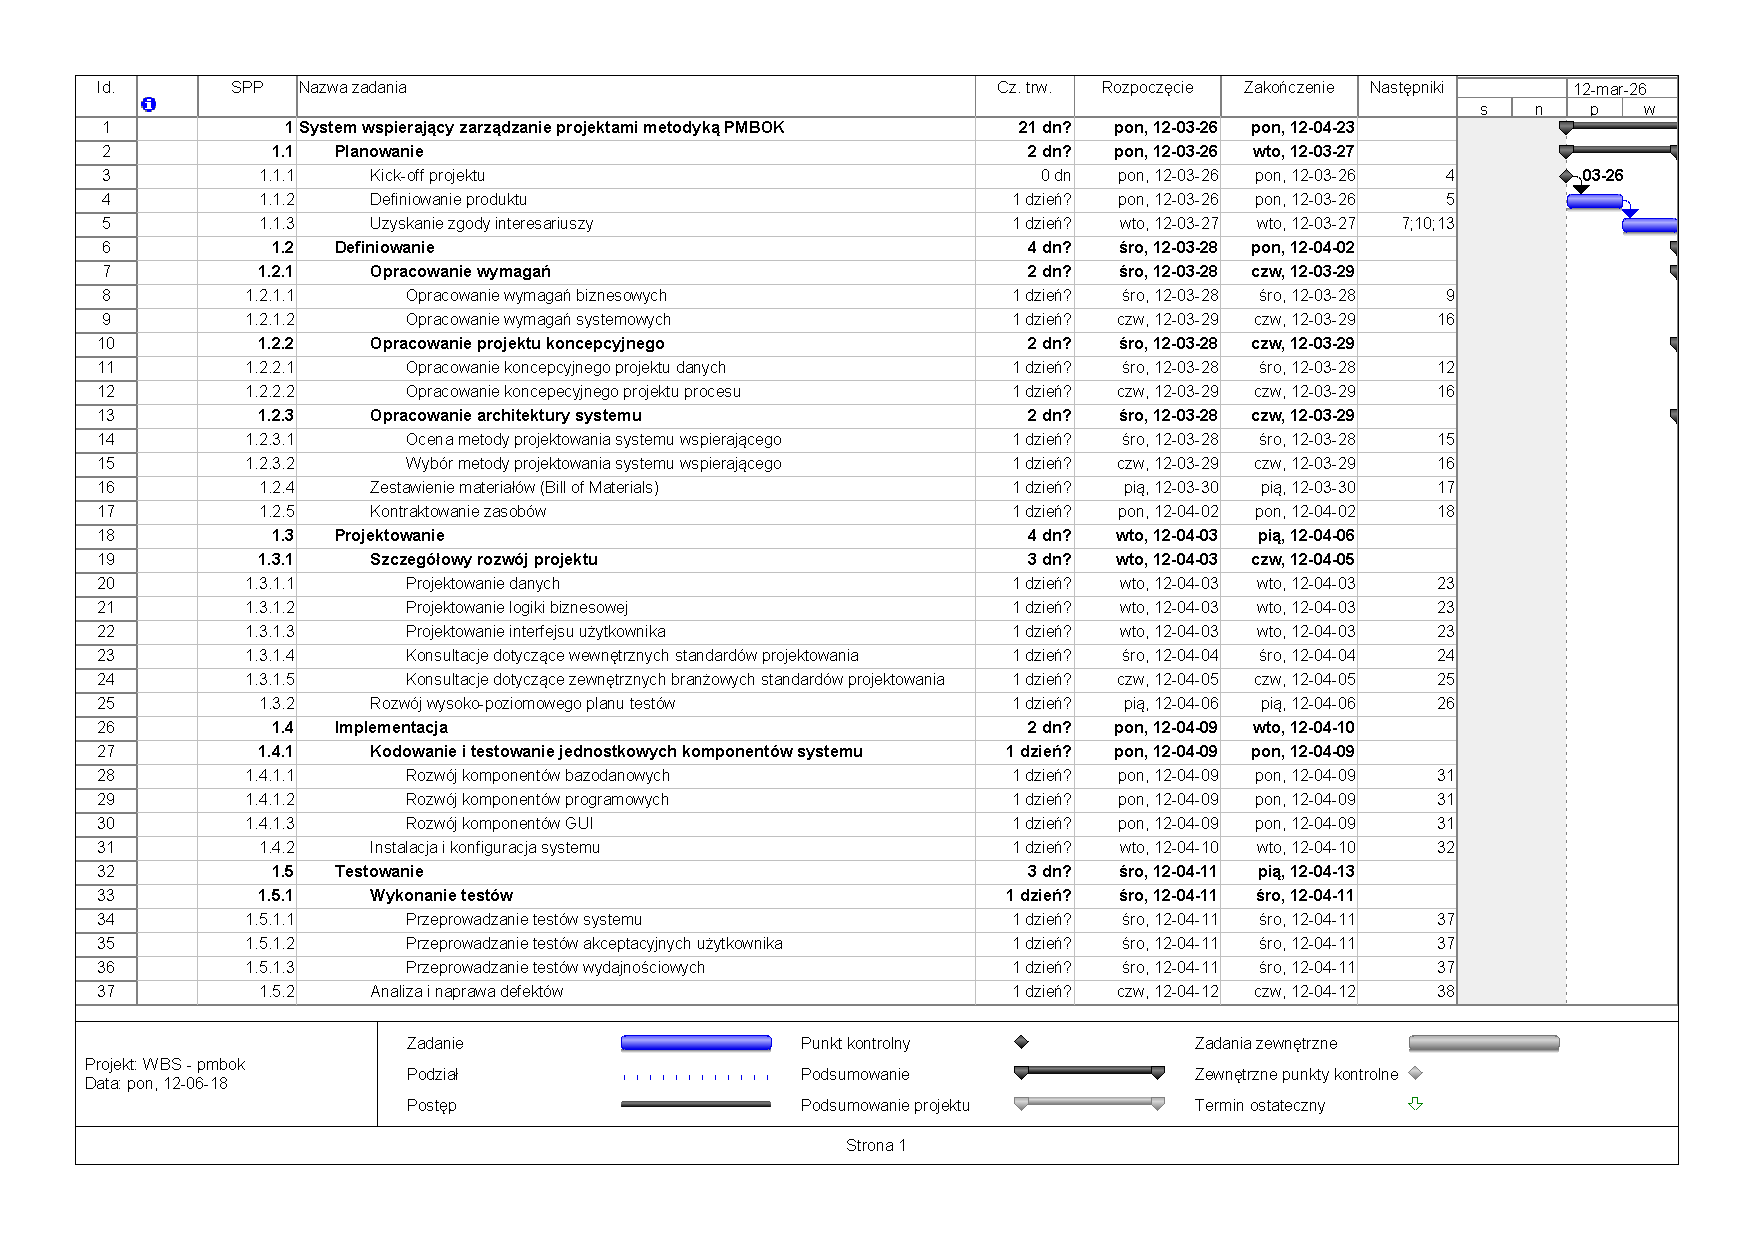
\includepdf[nup=2x2,pages=-,landscape=true,column=true]{harmonogramWBS.pdf}

% ===========================================================================

\section{Struktura RBS projektu}
% strona 45

\begin{figure}[htb]
\begin{center}
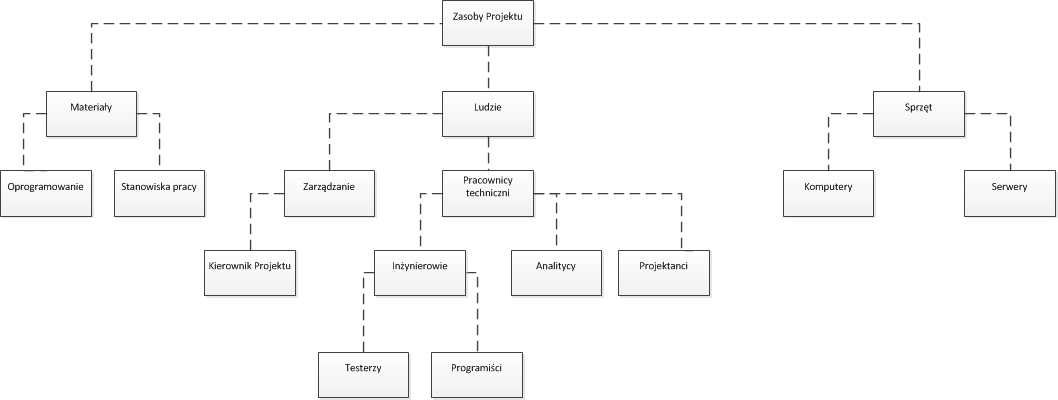
\includegraphics[width=\textwidth]{RBS.png}
\caption[RBS]{RBS}
\label{rysunekProces}
\end{center}
\end{figure}

% ===========================================================================

\section{Harmonogram z uwzględnieniem zasobów}
% strona 59

Ten wirtualny warsztat jest beznadziejny.



\chapter{Wykład 10. Zarządzanie kosztami w projekcie informatycznym}

\section{Plan poprawy procesu}
% strona 23

\textbf{I. Opracuj: plan poprawy procesu.}

\begin{enumerate}
\item Zapoczątkowanie poprawy procesu.
\begin{enumerate}

\item Definicja kontekstu oraz budżetu (sponsorowania) programu.
\item Ustalenie infrastruktury niezbędnej do doskonalenia procesu.
\end{enumerate}


\item Ocena dotychczas stosowanego procesu.
\item Identyfikacja obszarów procesu, które będą doskonalone.
\begin{enumerate}

\item Definicja strategii doskonalenia.
\item Podział zadań - "co, kto, jak i kiedy".
\item Implementacja procedury doskonalenia procesu.
\end{enumerate}


\item Zbadanie efektów procedury doskonalenia procesu.
\begin{enumerate}

\item Ponowna ocena procesu (w ograniczonym zakresie).
\item Analiza wyników początkowej oceny procesu z ponowną jego oceną.
\end{enumerate}

\item Walidacja procedury doskonalenia procesu wytwórczego.
\begin{enumerate}

\item Utrzymanie tempa i wyników procedury doskonalenia.
\item Formalne wprowadzenie procedury poprawy procesu do misji organizacji.

\end{enumerate}
\end{enumerate}



textbf{II.Wyznacz TCO i ROI.}

Koszty początkowe:
\begin{itemize}

\item kupno nowego sprzętu komputerowego – 4 000 zł,
\item koszty serwera do wersjonowania – 10 000 zł.
\end{itemize}

Koszty coroczne:
\begin{itemize}

\item serwis sprzętu – 1 000 zł,
\item cotygodniowe sprawdzanie i robienie backupów – 6 000zł.
\end{itemize}

Koszt przez  5 lat to 49 000 zł.
TCO rocznie:  9 800 zł.
\textbf{TCO miesięcznie:  817 zł.}
Przychód początkowy:
\begin{itemize}

\item szkolenie załogi - Koszt szkolenia 10 000 zł,
\item sprzedaż programu – 25 000 zł.
\end{itemize}

Przychód coroczny:
\begin{itemize}

\item przychód  z licencji - 7 000 zł,
\item serwis i upgrady – 10 000 zł.
\end{itemize}

Przychód wypracowany przez 5 lat: 120 000 zł.
Przychód rocznie : 24 000 zł.
Przychód miesięcznie: 2000 zł.
\textbf{Zysk netto: 2 000 zł – 817 zł = 1183 zł.}
\textbf{ROI:  1183\backslash817 * 100\% = 144,8\%} 

% ===========================================================================

\section{Plan zarządzania kosztami}
% strona 26

\textbf{I. Opracuj plan zarządzania kosztami.}

Zarządzanie kosztami:
\begin{enumerate}
\item Planowanie zasobów:
\begin{enumerate}
\item Struktura podziału pracy – opinie ekspertów.
\item Dane historyczne – określenie różnych wariantów realizacji.
\item Deklaracja zakresu – oprogramowanie wspierające zarządzanie projektami.
\item Opis puli zasobów.
\item Procedury organizacyjne.
\item Szacunki czasu trwania działań.
\end{enumerate}

\item Szacowanie kosztów:
\begin{enumerate}

\item WBS – szacowanie porównawcze.
\item Wymagania dotyczące zasobów – modelowanie parametryczne.
\item Ceny jednostkowe zasobów – szacowanie oddolne.
\item Szacunki czasu trwania działań.
\item Publikowane szacunki – inne metody szacowania.
\item Dane historyczne.
\item Plan kont
\item Dane o ryzykach.

\end{enumerate}

\item Budżetowanie kosztów:

\begin{enumerate}

\item Szacunki kosztów.
\item WBS.
\item Harmonogram projektu.
\item Plan zarządzania ryzykiem.

\end{enumerate}

\item Kontrola kosztów:
\begin{enumerate}
\item Plan bazowy kosztów – system kontroli zmian kosztów.
\item Raport z wykonania – pomiar wykonania.
\item Żądania zmian – technika zarządzania wartością wypracowaną.
\item Plan zarządzania kosztami – dodatkowe procesy planowania.
\end{enumerate}
\end{enumerate}



% ===========================================================================

\section{Wprowadzenie kosztów do planu projektu}
% strona 41

Tabela kosztów zaimportowana z programu MS Project:

\begin{figure}[!h]
\centering
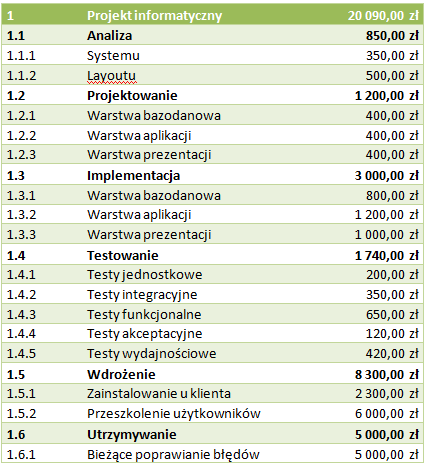
\includegraphics[width=1.1\textwidth]{tabelaKosztow.png}
\caption{Tabela kosztów}
\label{fig:tabelaKosztow}
\end{figure}

% ===========================================================================

\section{Monitorowanie projektu z wykorzystaniem EVA}
% strona 69

Poniższe wyliczenia zostały wykonane w programie MS Project, a nagłówki kolumn zostały nazwane polskimi odpowiednikami metody EVA (Earned Value Analysis) – wczesnej analizy wartości wypracowanej.

\begin{figure}[!h]
\centering
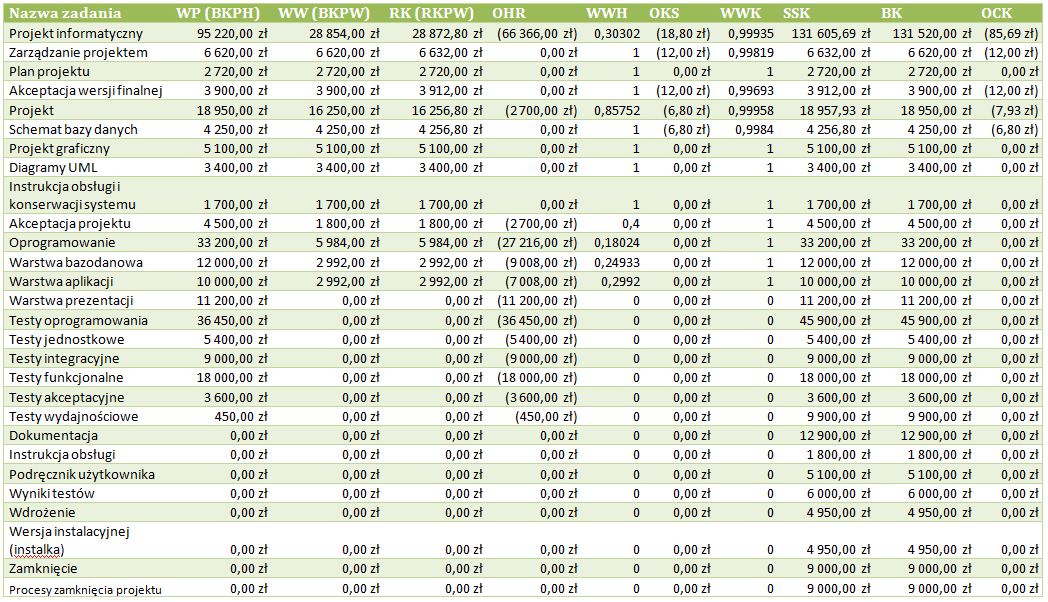
\includegraphics[width=1.1\textwidth]{monitorowanieEVA.png}
\caption{Monitorowanie projektu z wykorzystaniem EVA}
\label{fig:monitorowanieEVA}
\end{figure}

\chapter{Wykład 11. Zarządzanie jakością w projekcie informatycznym}

\section{Lista kontrolna}
% strona 38

\textbf{Obszar projektu:} ocena wiarygodności estymacji harmonogramu i kosztu projektu

\begin{figure}[h]
\begin{center}
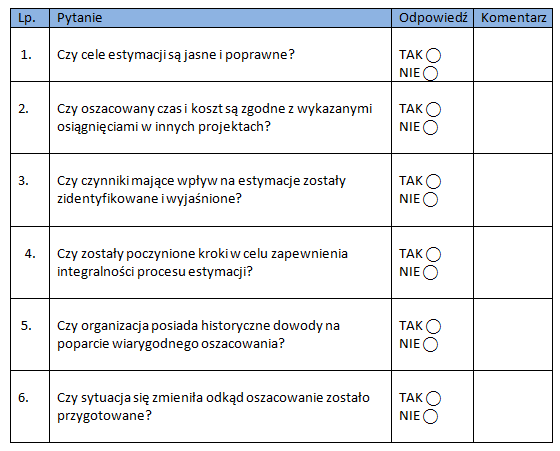
\includegraphics[scale=1]{checklist.png}
\caption[Lista kontrolna]{Lista kontrolna}
\label{rysunekProces}
\end{center}
\end{figure}

% ===========================================================================

\section{Plan poprawy procesów}
% strona 39

\textbf{Obszar projektu:} komunikacja

\textbf{Problem:} zespół nie może się dogadać, wymagania dotyczące projektu są błędnie interpretowane przez różne osoby, błędy jednej osoby pociągają za sobą błędy kolejnych, błędny przepływ informacji.

\textbf{Cel:} zgrany zespół, wymieniający się informacjami i problemami posiadający jasno określony cel działania znany wszystkim członkom zespołu

\begin{figure}[h]
\begin{center}
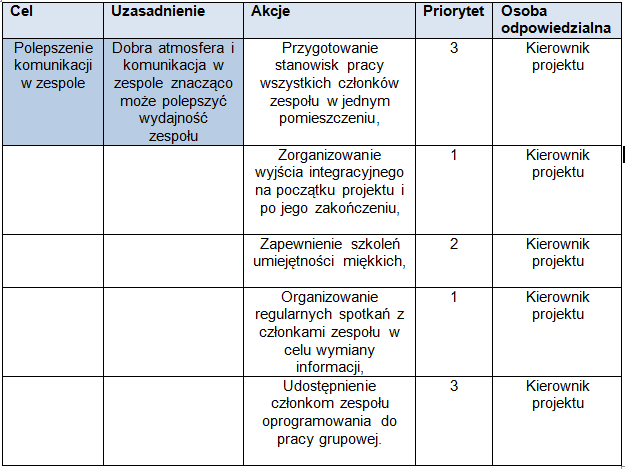
\includegraphics[scale=1]{planpoprawy.png}
\caption[Plan poprawy procesu]{Plan poprawy procesu}
\label{rysunekProces}
\end{center}
\end{figure}
 


% ===========================================================================

\section{Plan zarządzania jakością pod kątem przydziału zasobów}
% strona 56

\begin{enumerate}
\item	Przygotowanie listy wszystkich zasobów na podstawie RBS.
\item	Bieżąca ocena zasobów ludzkich pod kątem kwalifikacji i stanowiska.  Sprawdzenie czy pracownicy wypełniają swoje obowiązki zawarte w opisie stanowiska oraz czy ich kwalifikacje pozwalają na wykonywanie danych czynności.
\item	Kontrola czy zasoby nie są przeciążone – czy nie jest im przypisane zbyt dużo pracy do wykonania, czy nie są zbyt eksploatowane.
\end{enumerate}

% ===========================================================================

\section{Audyt jakości}
% strona 62

Ten wirtualny warsztat jest beznadziejny.

% ===========================================================================

\section{Wyniki procesu kontroli jakości}
% strona 68
Dzięki audytowi możliwa jest kontrola procesów mających miejsce w przedsiębiorstwie. Audyty pozwalają na wykrycie niedoskonałości i błędów w działaniu. Każdy naprawiony defekt i dostarczony produkt również musi przejść przez kontrolę jakości. 

Dokument wyniku procesu kontroli mógłby wyglądać w następujący sposób:

\begin{figure}[h]
\begin{center}
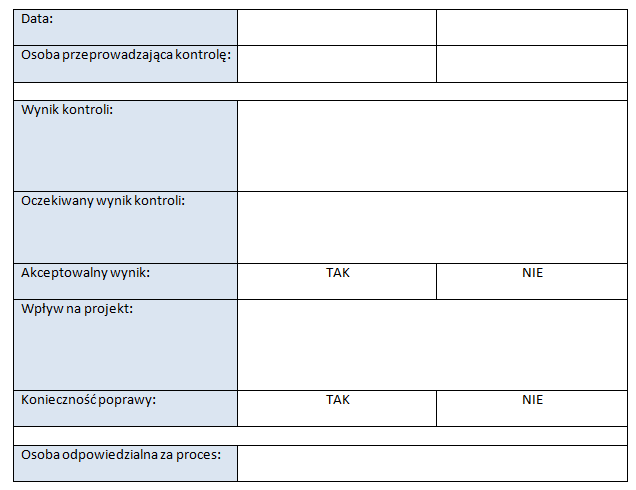
\includegraphics[scale=1]{wyniki.png}
\caption[Szablon dokumentu]{Szablon dokumentu}
\label{rysunekProces}
\end{center}
\end{figure}

% ===========================================================================

\section{Diagram przyczynowo-skutkowy w zarządzaniu jakością}
% strona 80

Diagram przyczynowo-skutkowy jest jednym z narzędzi doskonalenia jakości. Pozwala na zidentyfikowanie przyczyny problemu i ułatwia znaleznienie przyczyny źródłowej problemu (root cause). Etapy tworzenia:
\begin{enumerate}
\item	Identyfikacja problemu (szary prostokąt).
\item	Określenie głównych grup przyczyny (niebieskie prostokąty)
\item	Uszczegółowienie przyczyn 
\item	Analiza wyników.
\end{enumerate}

\begin{figure}[h]
\begin{center}
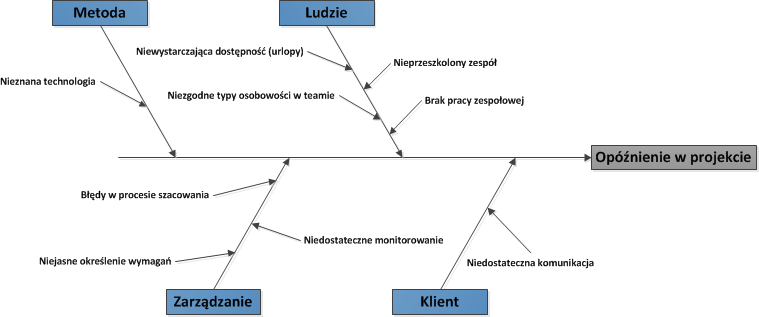
\includegraphics[scale=0.8]{ryba.png}
\caption[Diagram przyczynowo-skutkowy]{Diagram przyczynowo-skutkowy}
\label{rysunekProces}
\end{center}
\end{figure}



% ===========================================================================

\section{Diagram Pareto}
% strona 83

\begin{figure}[h]
\begin{center}
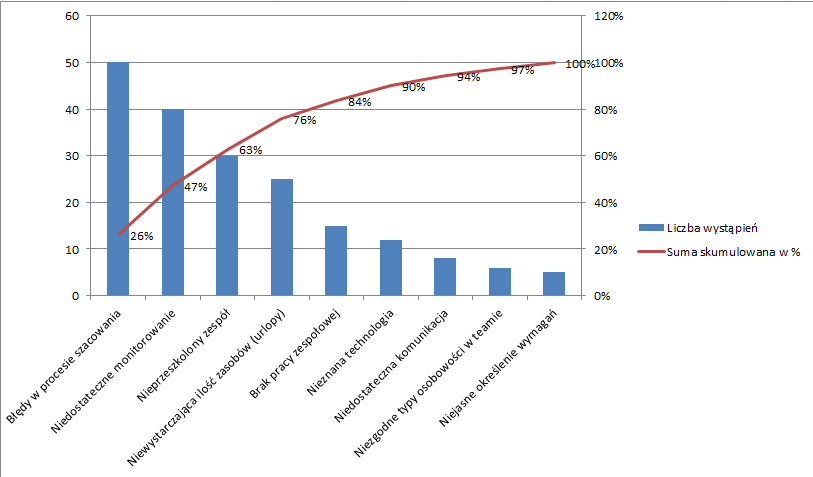
\includegraphics[scale=0.8]{pareto.png}
\caption[Diagram Pareto]{Diagram Pareto}
\label{rysunekProces}
\end{center}
\end{figure}


Czy zasada 20-80 się sprawdza?

W wykonanym przykładzie zasada 20-80 nie sprawdziła się.  Około 80\% problemów było generowanych przez ok 44\% przyczyn.




\chapter{Wykład 12. Zarządzanie zasobami ludzkimi w projekcie informatycznym}

\section{WBS i OBS}
% strona 20

\textbf{I. Opracuj powiązane WBS i OBS dla projektu.}

\begin{enumerate}
\item Projekt informatyczny

\begin{enumerate}

\item Analiza

\begin{enumerate}

\item Systemu
\item Layoutu

\end{enumerate}
\item Projektowanie

\begin{enumerate}

\item Warstwa bazodanowa
\item Warstwa aplikacji
\item Warstwa prezentacji

\end{enumerate}
\item Implementacja

\begin{enumerate}

\item Warstwa bazodanowa
\item Warstwa aplikacji
\item Warstwa prezentacji

\end{enumerate}
\item Testowanie

\begin{enumerate}

\item Testy jednostkowe
\item Testy integracyjne
\item Testy funkcjonalne
\item Testy akceptacyjne
\item Testy wydajnościowe

\end{enumerate}
\item Wdrożenie

\begin{enumerate}

\item Zainstalowanie u klienta
\item Przeszkolenie użytkowników

\end{enumerate}
\item Utrzymywanie

\begin{enumerate}

\item Bieżące poprawianie błędów

\end{enumerate}
\end{enumerate}
\end{enumerate}




\begin{enumerate}
\item Projekt informatyczny

\begin{enumerate}

\item Zarządzanie projektem

\begin{enumerate}

\item Plan projektu
\item Akceptacja wersji finalnej

\end{enumerate}

\item Projekt

\begin{enumerate}

\item Schemat bazy danych
\item Projekt graficzny
\item Diagramy UML
\item Instrukcja obsługi i konserwacji systemu

\end{enumerate}

\item Oprogramowanie

\begin{enumerate}

\item Warstwa bazodanowa
\item Warstwa aplikacji
\item Warstwa prezentacji

\end{enumerate}

\item Testy oprogramowania

\begin{enumerate}

\item Testy jednostkowe
\item Testy integracyjne
\item Testy funkcjonalne
\item Testy akceptacyjne
\item Testy wydajnościowe

\end{enumerate}

\item Dokumentacja

\begin{enumerate}

\item Instrukcja obsługi
\item Podręcznik użytkownika
\item Wyniki testów

\end{enumerate}

\item Wdrożenie

\begin{enumerate}

\item Wersja instalacyjnej (instalka)

\end{enumerate}
\end{enumerate}
\end{enumerate}



\textbf{II. Przedstaw macierz RAM RACI dla projektu.}

R – odpowiedzialny, C – konsultowany, A – zatwierdzający, I – informowany

\begin{figure}[!h]
\centering
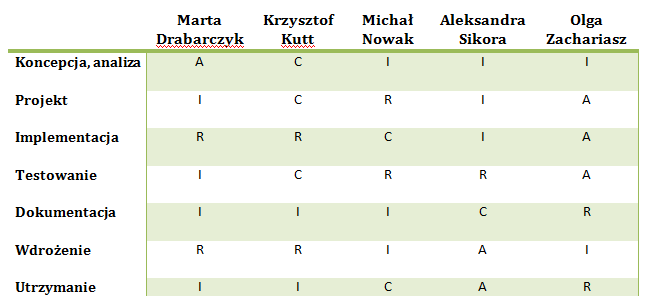
\includegraphics[width=1.1\textwidth]{macierzRAM.png}
\caption{Macierz RAM RACI dla projektu}
\label{fig:macierzRAM}
\end{figure}


% ===========================================================================

\section{Sposób wykorzystania integracji}
% strona 21

\textbf{I. Opracuj w jaki sposób wykorzystasz integrację dla realizacji celu projektu.}
Zarządzanie integracją projektu zapewnia procesy, które mają za zadanie zapewnić, że elementy znajdujące się w procesie są koordynowane poprawnie. Do jego zadań należy też dokonywanie wyboru pomiędzy przewyższaniem oczekiwań a celami ich zaspakajania oraz wymaganiami ich udziałowców.
Do głównych procesów należą:

\begin{itemize}
\item tworzenie planu projektu,
\item wykonywanie planu projektu,
\item ogólny nadzór zmian.
\end{itemize}

Poszczególny proces działa wspólnie z innymi procesami, każdy z nich chociaż raz występuje we wszystkich fazach projektu.
Tworzymy plan projektu - zbiorczy dokument, który jest robiony na podstawie innych dokonanych rezultatów w procesach planowania. Używa się go jako przewodnika do tworzenia projektu jak również do jego kontrolowania.
Elementy przedstawienia planu projektów:

\begin{itemize}
\item karta projektu,
\item zakres,
\item zapis struktury pracy,
\item prowadzenie terminów i kosztów,
\item główne kamienie milowe oraz ich terminy,
\item główny lub wymagany personel,
\item główne czynniki ryzyka,
\item plan zakresu lub terminu,
\item trudne do rozwiązania problemy lub oczekujące na realizacje decyzje.
\end{itemize}

Inne elementy informacyjne zawiera się planie a jest to zależne od potrzeb i wymagań specyfiki projektu.
Wykonujemy plan projektu. Jest to podstawy proces który ma na celu realizację planu do którego wykorzystuje się większość zaplanowanego na projekt budżetu.
Nadzorujemy zmiany - proces związany z zmianami, które przynoszą oczekiwane korzyści przy wpływie na czynniki, zapewniają następowanie po sobie zmian i następnie ich zarządzeniem poprzez mierzenie stopnia realizacji, który ma na celu wpłynąć na wszystkie zmiany w planie, 
a następnie zmiany wpłyną na zasady.



% ===========================================================================

\section{Zasady stosowania pracy zdalnej}
% strona 29

textbf{I. Opracuj zasady stosowania pracy zdalnej (tele-pracy) w Twoim projekcie.}

Zasady stosowania pracy zdalnej w naszym projekcie:
\begin{itemize}
\item regularny przepływ informacji w obrębie zespołu wirtualnego,
\item komunikacja powinna odbywać się na bieżąco,
\item komunikaty powinny jasno przedstawiać pogląd na daną kwestie i  być poprzedzone wcześniejszymi uzgodnieniami,
\item każdy członek zespołu ma jasno określone zadanie,
\item pracujemy według określonego harmonogramu,
\item wszyscy członkowie zespołu muszą dotrzymywać terminów,
\item stosujemy oprogramowanie typu unified messaging - integrujące komunikację faksową, telefoniczną i e-mailową oraz pakiety wspierające pracę grupową,
\item używamy oprogramowania umożliwiającego przejmowanie zdalnej kontroli z domu nad komputerami znajdującymi się w biurze.

\end{itemize}


% ===========================================================================

\section{Zasady nagradzania}
% strona 46

{I. Opracuj zasady nagradzania w Twoim projekcie i opisz jak to nagradzanie będzie miało wpływ na wykonanie projektu i przez jak długi czas.}

Zasady nagradzania:

\begin{itemize}
\item docenianie wykonanej pracy,
\item należy większą wagę przykładać do sukcesów kolegów niż do ich porażek,
\item uznanie powinno być wygłoszone publicznie, tak aby inny członkowie zespołu je usłyszeli,
\item nagroda czy pochwała powinna być przekazana osobiście, a nie np. mailowo,
\item nagradzanie powinno mieć urozmaicone formy,
\item nagroda powinno zostać przyznana w miarę szybko,
\item osiągnięcia powinny kojarzyć się z nagradzaniem.
\end{itemize}
Nagradzanie może podnieść jakość wykonywanej pracy oraz zmobilizować zespół do jak najszybszego skończenia projektu. Natomiast głównym celem grupy projektowej jest uzyskanie pozytywnej oceny 
z przedmiotu, więc jakiekolwiek motywowanie będzie miało szanse oddziaływać do tego właśnie momentu.


% ===========================================================================

\section{Zasady motywowania}
% strona 72

W naszym zespole projektowym zostaną zastosowane następujące zasady motywacji:
\begin{itemize}
\item Motywowowanie poprzez pokazanie członkom zespołu, że ich wkład do projektu jest rzeczywisty i wykorzystywany
\item Wynagradzanie pracowników zgodnie z ich osiągnięciami
\item Jako korzyści brzegowe zastosujemy m.in. podział zysku, ubezpieczenie, możliwość dalszego rozwoju poprzez szkolenia zewnętrzne, różnego rodzaju karty umożliwiające darmową aktywność sportową, prywatna opieka zdrowotna
\item W naszej firmie będzie wykorzystywany głównie model Kierownika Y (kierownik typu X wprowadzany w sytuacjach krtycznych)
\item Zapewnienie dobrych warunków higienicznych zgodnie z teorią Herzberga, w celu uniknięcia obniżenia motywacji
\item Stosowanie różnych form premii oraz awansów
\item Publiczne pokazywanie uznania dla najlepszych pracowników
\item Zwiększanie odpowiedzialności w przypadku najlepszych pracowników
\item Dbanie o organizację pracy oraz dobre kontakty między pracownikami
\end{itemize}


% ===========================================================================

\section{Role w zespole projektowym}
% strona 83

\textbf{I. Przeprowadź analizę Twojego zespołu projektowego pod względem ról w zespole.}

Role poszczególnym członkom zespołu zostały przydzielone na podstawie wyników testu przeprowadzonego na zajęciach.

\begin{figure}[!h]
\centering
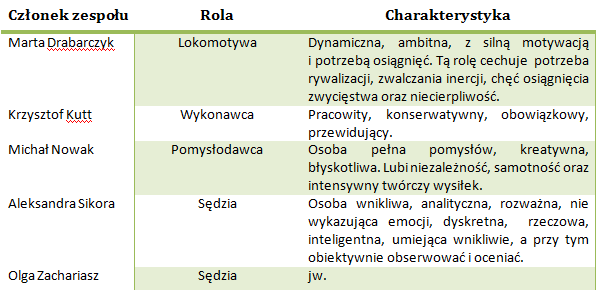
\includegraphics[width=1.1\textwidth]{roleWZespole.png}
\caption{Role w zespole projektowym}
\label{fig:roleWZespole}
\end{figure}

\textbf{II. Przedstaw możliwe rozwiązania.}

Nasz zespół pod względem posiadania ról w zespole jest dość zróżnicowany, niemniej jednak dołączenie się osób posiadających role „koordynatora” czy też „duszy zespołu” byłoby dla nas plusem.



\chapter{Wykład 13. Zarządzanie komunikacją w projekcie informatycznym}

\section{Interesariusze projektu}
% strona 29

Ten wirtualny warsztat jest beznadziejny.

% ===========================================================================

\section{Plan przekazywania informacji}
% strona 40

\textbf{I. Opracuj plan przekazywania informacji w projekcie.}

Przekazywanie informacji w projekcie: 

\begin{figure}[!h]
\centering
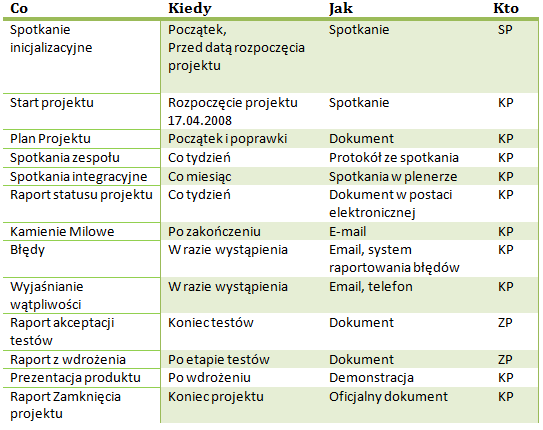
\includegraphics[width=1.1\textwidth]{przekazywanieInformacji.png}
\caption{Plan przekazywania informacji}
\label{fig:przekazywanieInformacji}
\end{figure}

Przekazywanie innym osobom informacji o projekcie:
 Do przekazywania informacji o projekcie (udziałowcom lub osobom, którym przydzielono pracę) można skorzystać z takich funkcji jak:
\begin{itemize}
\item Drukowanie i raportowanie, aby przedstawić innym informacje o projekcie na papierze. 
\item Publikowanie w formacie HTML lub zapisywanie planu projektu na serwerze sieci Web, aby dać innym dostęp do informacji o projekcie w witrynie sieci Web. 
\item Program Microsoft Project Central lub grupy robocze, aby używać programu Microsoft Project Central zainstalowanego w firmowej sieci intranet lub w Internecie albo systemu poczty e-mail w celu przekazywania innym informacji o projekcie. 
\item Integracja z programem Microsoft Outlook, aby inne osoby przeglądały zadania na swoich listach zadań programu Outlook.
\end{itemize}


% ===========================================================================

\section{Szablon spotkania i notatki ze spotkania}
% strona 65

Ten wirtualny warsztat jest beznadziejny.



\chapter{Wykład 14. Zarządzanie ryzykiem w projekcie informatycznym}

\section{Macierz ryzyka}
% strona 27

Zidentyfikowane ryzyka:
\begin{enumerate} %nie zmieniać kolejności, bo te liczby są w tabeli!
\item Nieznajomość wybranego w projekcie języka programowania
\item Niedyspozycja członka zespołu (choroba, awaria sprzętu)
\item Awaria repozytorium (svn)
\item Skrócenie czasu realizacji projektu
\item Klęska żywiołowa
\item Problemy merytoryczne związane z brakiem doświadczenia w tematyce projektu
\item Niespełnienie wymagań jakościowych (błędne działanie na różnych systemach operacyjnych, wolne działanie aplikacji, zawodność)
\item Zbyt długi czas realizacji projektu
\item Skończenie się środków z odszkodowania które zostały przeznaczone na projekt
\item Niemożliwość znalezienia kupca chętnego na projekt po jego zakończeniu
\item Odejście przed zakończeniem projektu, któregoś z członków grupy projektowej
\item Otrzymanie innego dużego zlecenia w trakcie prac nad dokończeniem projektu
\item Przedłużający się proces z inwestorem w sprawie odszkodowania
\item Ukazanie się we wcześniejszym terminie produktu konkurencyjnej firmy
\item Wewnętrzna sytuacja w firmie zmuszająca do przeznaczenia środków z odszkodowania na inne cele
\item Pomimo znalezienia klientów inwestycja nie zwraca się
\end{enumerate}


\begin{table}[htb]
\centering
\begin{tabular}{|c|c|c|c|c|c|c|} 
\multicolumn{3}{|c|}{Szanse} &  & \multicolumn{3}{|c|}{Zagrożenia} \\
\hline  &  &  & Mocny & 1,10,11 & 3,7,9 &  \\
\hline  & 4 &  & Umiarkowany & 5,14,15 & 2,6,8 & 13 \\
\hline  &  &  & Słaby &  & 12,16 &  \\
\hline Wysokie & Średnie & Niskie &  & Niskie & Średnie & Wysokie \\
\end{tabular}
\caption{\textbf{Macierz prawdopodobieństwa dyskretna (trój-poziomowa)}. \mbox{\textit{Prawodopodobieństwo:}} oś pozioma,  \textit{Wpływ:} oś pionowa}
\label{tab:macierzPrawdopodobienstwa}
\end{table}


\begin{table}[htb]
\centering
\begin{tabular}{|c|c|c|c|} 
\hline Mocny & III & IV & V \\
\hline Umiarkowany & II & III & IV \\
\hline Słaby & I & II & III \\
\hline & Niskie & Średnie & Wysokie \\
\end{tabular}
\caption{\textbf{Poziomy ryzyka}}
\label{tab:poziomyRyzyka}
\end{table}


Definicje poziomów ryzyka:
\begin{enumerate}[I]
\item \textbf{Ryzyko tolerowane}. Posiada mały lub żaden efekt na cele projektu. Prawdopodobieństwo jest na tyle małe, że nie ma potrzeby ich rozpatrywania.
\item \textbf{Ryzyko małe}. Mały wpływ na cele projektu. Prawdopodobieństwo wystąpienia małe w
związku z tym niezbyt duża koncentracja nad ryzykiem.
\item \textbf{Ryzyko średnie}. Może wpłynąć na cele projektowe, harmonogram i koszty. Prawdopodobieństwo pojawienia się jest na tyle wysokie, że musi podlegać ścisłej kontroli wszystkich czynników wpływających na ryzyko.
\item \textbf{Ryzyko wysokie}. Wysokie prawdopodobieństwo pojawienia się, wpływające na cele projektu, koszt i harmonogram. Ryzyko musi podlegać ścisłej kontroli określenia akcji zapobiegawczych.
\item \textbf{Ryzyko nietolerowane}. To ryzyko należy do najważniejszych zagrożeń i szans w projekcie.
\end{enumerate}


% ===========================================================================

\section{Rejestr ryzyka projektowego}
% strona 36

Ten wirtualny warsztat jest beznadziejny.

% ===========================================================================

\section{Analiza jakościowa i ilościowa SWOT}
% strona 48

\begin{figure}[h]
\begin{center}
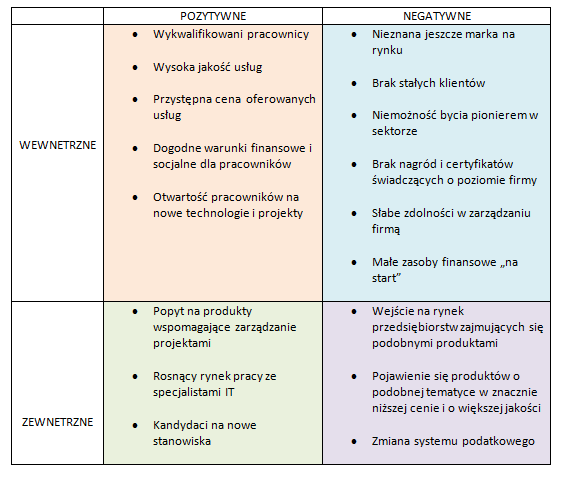
\includegraphics[scale=1]{swot.png}
\caption[Analiza SWOT]{Analiza SWOT}
\label{rysunekProces}
\end{center}
\end{figure}

\clearpage

% ===========================================================================

\section{Analiza jakościowa ryzyka}
% strona 54

Na pół roku przed końcem projektu, inwestor wycofuje się z projektu, zarzucając go.
\begin{itemize}
\item zgodnie z zapisem w umowie otrzymujemy 200 000 tys zł odszkodowania, za zerwanie umowy
\item postanawiamy dokończyć projekt w przeciągu pół roku, a następnie znaleźć chętnych na niego klientów
\item PMBOK jest popularny, więc powinniśmy znaleźć przedsiębiorstwo które pracuje zgodnie z nim
\item Zarzucenie projektu, który jest w wysokim stopniu zaawansowania prac jest nieopłacalne
\end{itemize}


Prawdopodobieństwo:  M - małe, S – średnie, D – duże\\
Wpływ: N - niski, P – poważny, W – wielki

\begin{table}[htb]
\centering
\begin{tabular}{|c|p{11.5cm}|c|c|} 
\hline Lp. & Opis & Prawdop. & Wpływ \\
\hline 1 & Zbyt długi czas realizacji projektu & S & P \\
\hline 2 & Skończenie się środków z odszkodowania które zostały przeznaczone na projekt & S & W \\
\hline 3 & Niemożliwość znalezienia kupca chętnego na projekt po jego zakończeniu & M & W \\
\hline 4 & Odejście przed zakończeniem projektu, któregoś z członków grupy projektowej & M & W \\
\hline5 & Długotrwała choroba kogoś z grupy projektowej & S & P \\
\hline6 & Otrzymanie innego dużego zlecenia w trakcie prac nad dokończeniem projektu & S & N \\
\hline7 & Przedłużający się proces z inwestorem w sprawie odszkodowania & D & P \\
\hline8 & Ukazanie się we wcześniejszym terminie produktu konkurencyjnej firmy & M & P \\
\hline9 & Wewnętrzna sytuacja w firmie zmuszająca do przeznaczenia środków z odszkodowania na inne cele  & M & P  \\
\hline10 & Pomimo znalezienia klientów inwestycja nie zwraca się &  S & N  \\
\hline
\end{tabular}
\caption{\textbf{Analiza jakościowa ryzyka}}
\label{tab:analizaJakosciowa}
\end{table}

\clearpage

\begin{table}[!h]
\centering
\begin{tabular}{|c|c|c|c|} \hline Prawdop. \textbackslash Wpływ & Niski & Poważny & Wielki \\
 \hline Duże &  & 7 &  \\
\hline Średnie & 6,10 & 1,5 & 2 \\
\hline Małe &  & 8,9  & 3,4  \\
\hline
\end{tabular}
\caption{\textbf{Macierz prawdopodobieństwa}}
\label{tab:macierzPrawdopodobienstwa}
\end{table}




% ===========================================================================

\section{Analiza ilościowa ryzyka}
% strona 62

\begin{table}[htb]
\centering
\begin{tabular}{|c|p{7.0cm}|c|c|c|c|}
\hline 
Lp. & Opis & Prawdop. & Kwota & Wart. efektu finans. \\
 \hline 1 & Zbyt długi czas realizacji projektu & 25\% & 200 000 zł  & 50 000 zł \\
\hline 2 & Skończenie się środków z odszkodowania które zostały przeznaczone na projekt & 10\% & 150 000 zł & 15 000 zł \\
\hline 3 & Długotrwała choroba kogoś z grupy projektowej &  30\%  & 30 000 zł & 10 000 zł \\
\hline 4 & Przedłużający się proces z inwestorem w sprawie odszkodowania & 50\% & 50 000 zł & 25 000 zł \\
\hline 5 & Wewnętrzna sytuacja w firmie zmuszająca do przeznaczenia środków z odszkodowania na inne cele  & 5\% & 150 000 zł & 7 500 zł  \\
\hline6 & Pomimo znalezienia klientów inwestycja nie zwraca się &  30\% & 100 000 zł & 30 000 zł  \\
\hline
\end{tabular}
\caption{\textbf{Analiza ilościowa ryzyka}}
\label{tab:analizaIlosciowa}
\end{table}

\clearpage

% ===========================================================================

\section{Plany reakcji na ryzyko}
% strona 75

\begin{figure}[h]
\begin{center}
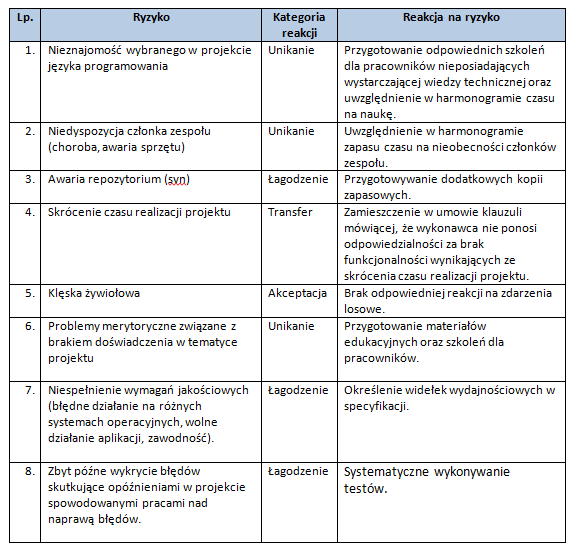
\includegraphics[width=\textwidth]{planreakcji.png}
\caption[Plan reakcji na ryzyko]{Plan reakcji na ryzyko}
\label{rysunekProces}
\end{center}
\end{figure}



\chapter{Wykład 15. Zarządzanie kontraktami w projekcie informatycznym}

\section{Formy wynajmu prac}
% strona 13

Z powodu niewielkich rozmiarów naszej firmy, a także braku specjalistów z niektórych dziedzin postanowiliśmy zlecić część zadań innym firmom. Dwa główne zadanie z którymi związane będzie zlecenie prac to opracowanie i stworzenie szaty graficznej dla naszego produktu, a także zapewnienie oraz utrzymanie serwerów na potrzeby naszego przedsiębiorstwa. Dla naszej firmy proponujemy następujące formy wynajmu prac:
\begin{itemize}
\item Najlepsze osiągalne rozwiązania (best-of-breed) – w każdym obszarze planujemy rozważyć zlecenie zadań związanych z nim na zewnątrz, albo pozostawienie ich wewnątrz firmy. Kupowanie rozwiązań dla różnych obszarów od różnych firm pozwoli nam zapewnić najlepsze dla przedsiębiorstwa rozwiązanie.
\item Partnerstwo – zawarcie umowy z inną firmą zajmującą się szeroko pojętą grafiką, pozwoli nam zapewnić szatę graficzną naszego produktu na wysokim poziomie, a także przetransferować ryzyko związane z brakiem grafików w naszym zespole.
\item Outsourcing – planujemy oddelegować do zewnętrznej firmy zadań związanych z dostarczeniem i utrzymaniem serwera na potrzeby naszego przedsiębiorstwa.
\end{itemize}

% ===========================================================================


\section{Szkic kontraktu}
% strona 31

\begin{figure}[!h]
\centering
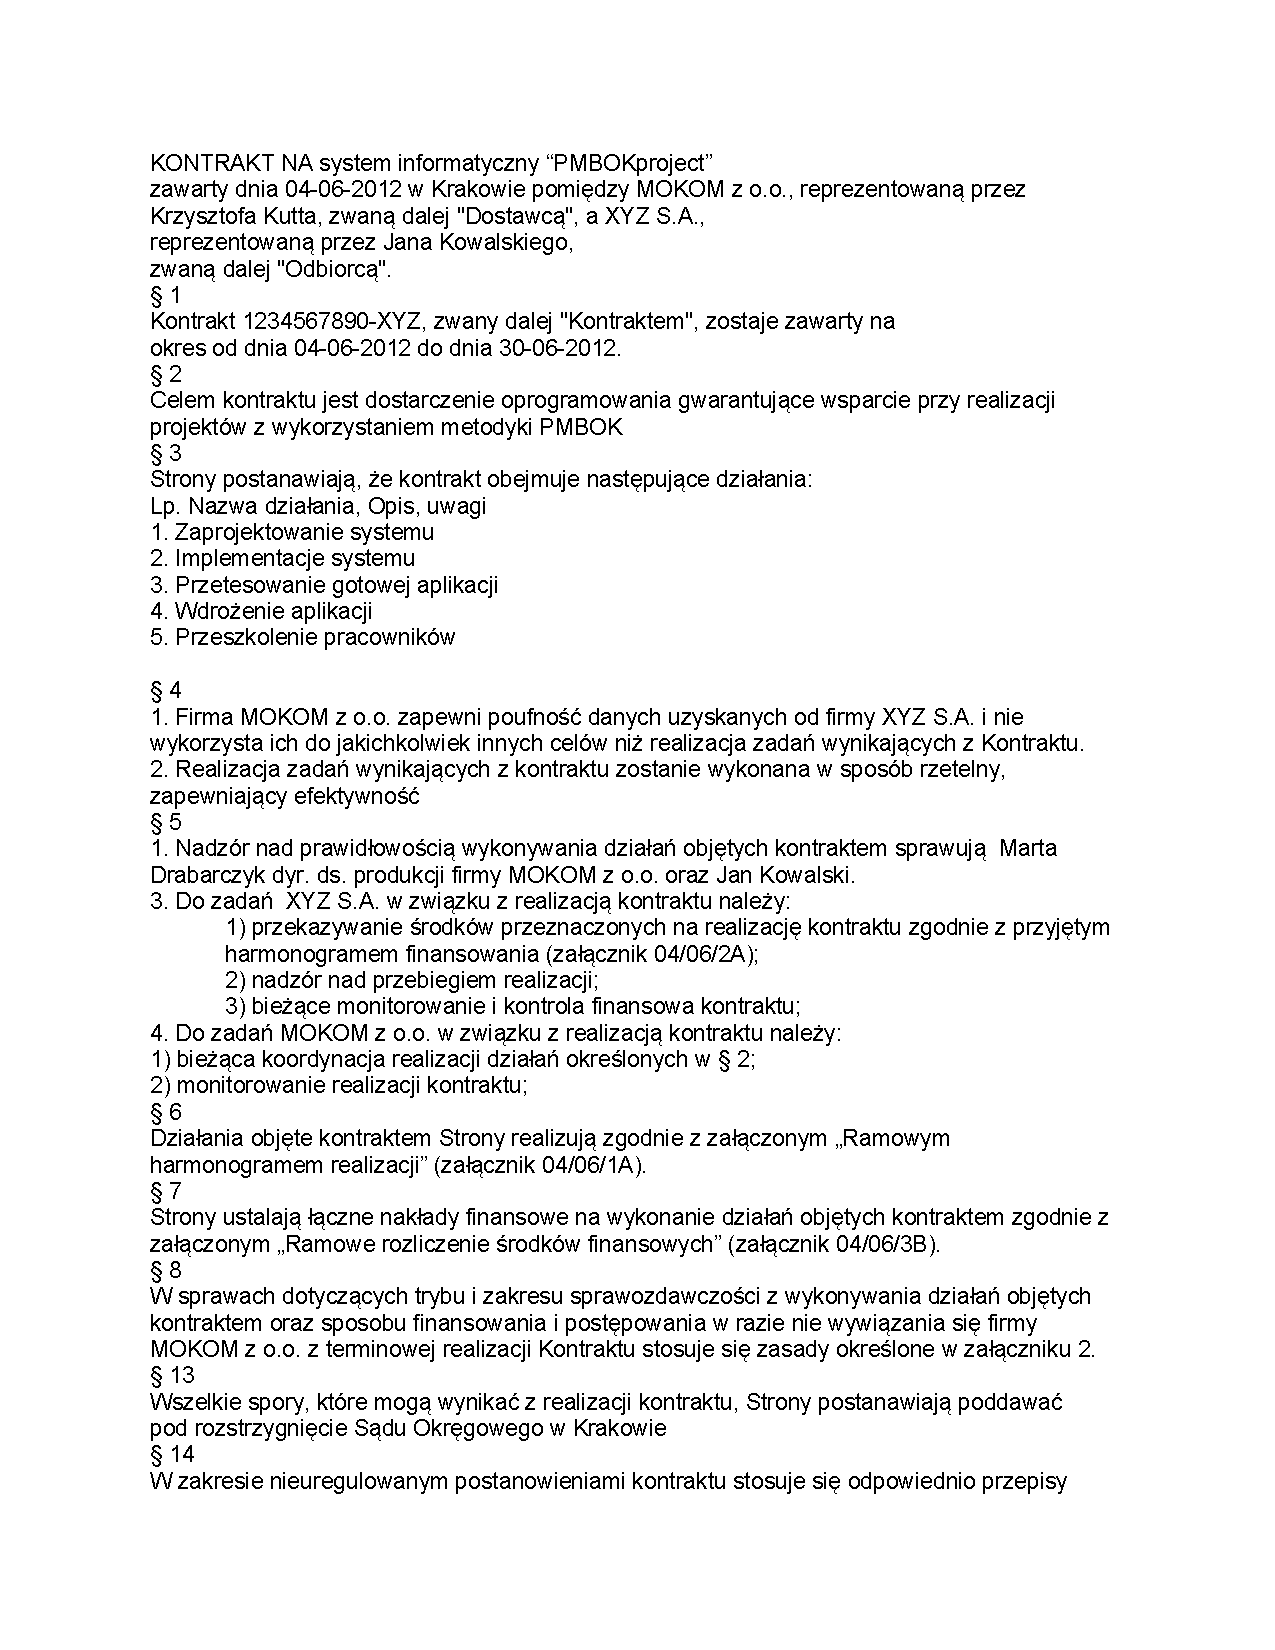
\includegraphics[width=1.1\textwidth]{szkicKontraktu.pdf}
\caption{Szkic kontraktu}
\label{fig:szkicKontraktu}
\end{figure}

% ===========================================================================

\section{Wybór prac, które należy zlecić. Wybór dostawcy}
% strona 50

Ten wirtualny warsztat jest beznadziejny.

% ===========================================================================

\section{Wybór kontraktu dla organizacji oraz podwykonawców}
% strona 50

Ten wirtualny warsztat jest beznadziejny.


\end{document}

